\documentclass[11pt,a4paper]{article}

% ======================= PAQUETES =======================
\usepackage[utf8]{inputenc}
\usepackage[T1]{fontenc}
\usepackage[spanish]{babel}
\usepackage[a4paper,margin=2.2cm]{geometry}
\usepackage{graphicx}
\usepackage{xcolor}
\usepackage{booktabs}
\usepackage{longtable}
\usepackage{array}
\usepackage{hyperref}
\usepackage{url}
\usepackage{fancyhdr}
\usepackage{titlesec}
\usepackage{enumitem}
\usepackage{caption}
\usepackage{amsmath}
\usepackage{tabularx}
\usepackage{tikz}
\usetikzlibrary{positioning}
\usetikzlibrary{shapes.geometric}
\usetikzlibrary{calc}
\usetikzlibrary{arrows.meta}

% ======================= COLORES INSTITUCIONALES =======================
\definecolor{uteqgreen}{RGB}{0,102,68}
\definecolor{uteqgray}{RGB}{90,90,90}

% ======================= HIPERVÍNCULOS =======================
\hypersetup{
    colorlinks=true,
    linkcolor=uteqgreen,
    citecolor=uteqgreen,
    urlcolor=blue,
    pdftitle={Documento Evidencia MDD - Modelio - AquaGest},
    pdfauthor={Equipo AquaGest - UTEQ}
}

% ======================= ENCABEZADOS =======================
\pagestyle{fancy}
\fancyhf{}
\renewcommand{\headrulewidth}{0.4pt}
\fancyhead[L]{\small Ingeniería de Requisitos (ISR-401) -- UTEQ}
\fancyhead[R]{\small MDD con Modelio -- Proyecto AquaGest}
\fancyfoot[C]{\thepage}

% ======================= TÍTULOS =======================
\titleformat{\section}{\large\bfseries\color{uteqgreen}}{\thesection}{1em}{}
\titleformat{\subsection}{\normalsize\bfseries\color{uteqgray}}{\thesubsection}{1em}{}
\titlespacing*{\section}{0pt}{1.4ex plus 0.5ex minus .2ex}{0.8ex plus .2ex}
\titlespacing*{\subsection}{0pt}{1.1ex plus 0.4ex minus .2ex}{0.5ex plus .1ex}

\setlength{\parskip}{0.35em}
\setlength{\parindent}{0pt}

\title{}
\date{}

\begin{document}

% ======================= CARÁTULA =======================
\begin{titlepage}
\centering
\vspace*{0.5cm}

{\Large \bfseries UNIVERSIDAD TÉCNICA ESTATAL DE QUEVEDO}\\[0.3cm]
{\large Facultad de Ciencias de la Computación y Diseño Digital}\\
{\large Carrera de Ingeniería en Software}\\[1.2cm]


\vspace{1.2cm}
{\large \bfseries DOCUMENTO EVIDENCIA}\\[0.2cm]
{\large Exposición con demostración práctica}\\[0.4cm]

{\Large \bfseries ``Herramientas que generan código fuente a partir de modelos UML''}\\[0.3cm]
{\large Ciclo completo Model-Driven Development (MDD) aplicado al Proyecto Fin de Curso (PFC)}\\[0.6cm]

{\large \bfseries Herramienta seleccionada: MODELIO}\\[1cm]

{\large \bfseries Caso de aplicación:}\\
{\large AquaGest -- Sistema para la Gestión Inteligente de una Camaronera}\\[1.2cm]

\begin{tabular}{ll}
\textbf{Asignatura:} & Ingeniería de Requisitos (ISR-401) \\
\textbf{Docente:} & Ing. Gleiston Guerrero Ulloa, PhD. \\
\textbf{Período académico:} & 2026--2027 PPA \\
\textbf{Paralelo:} & 4to ``A'' Software \\
\end{tabular}

\vspace{1cm}
{\bfseries Integrantes:}\\
Amagua Sacon Robyn Willian\\
Crespo Espinoza Kleber Obed\\
Rizzo Velez Edson Nagib\\


\vspace{0.6cm}
{\bfseries Repositorio GitHub de la actividad MDD (PFC-AquaGest-MDD-Equipo):}\\
\vspace{1.0cm}
\sloppy \url{https://github.com/erizzov-boop/PFC-AquaGest-MDD-Equipo_D-}

\vfill
{\large Quevedo, Ecuador -- 2026--2027 PPA}
\end{titlepage}

\newpage

% ======================= TABLA DE CONTENIDO =======================

\tableofcontents
\newpage

% ======================= RESUMEN =======================
\section*{Resumen}
\addcontentsline{toc}{section}{Resumen}

Este documento evidencia la exposición-demostración ``Herramientas que generan
código fuente a partir de modelos UML'' de Ingeniería de Requisitos (ISR-401),
UTEQ. El problema abordado es la ausencia, en el proceso actual del equipo, de
un mecanismo automatizado que derive código Java desde los modelos UML del
Proyecto Fin de Curso (PFC) \textbf{AquaGest}, sistema de gestión inteligente
para una camaronera. La herramienta seleccionada es \textbf{Modelio} (código
abierto), con su módulo Java Designer.

El caso de aplicación es el subsistema \textbf{Control de Estanques, Siembras y
Seguimiento}, modelado con seis clases (\texttt{Estanque}, \texttt{Siembra},
\texttt{Empleado}, \texttt{SobrecargaSiembra}, \texttt{Grameo},
\texttt{AlertaCrecimiento}) sobre RF-01 a RF-08 y RF-17, complementado con
diagramas de casos de uso y de estados. El equipo construyó y validó el modelo
(0 errores, 0 advertencias), generó código Java para las seis clases, verificó
directamente el contenido de dos de ellas -- confirmando que el generador
respeta la navegabilidad y multiplicidad de las asociaciones del modelo --, y
ejecutó un \textit{roundtrip} controlado que confirmó que el generador
sobrescribe el código sin preservar cambios manuales. Quedan pendientes:
inspeccionar las cuatro clases restantes, el registro de commits por
integrante y la exposición en vivo.





% ======================= MARCO TEÓRICO =======================
\section{Marco teórico}
\label{sec:marco-teorico}

\subsection{Model-Driven Engineering (MDE)}
El paradigma de Ingeniería Dirigida por Modelos (\textit{Model-Driven Engineering},
MDE) plantea que los modelos son artefactos de primera clase del desarrollo: el
modelo es la fuente autoritativa del sistema, y las implementaciones se derivan de
él mediante transformaciones automatizadas en lugar de escribirse manualmente
\cite{schmidt2006,bucchiarone2020}.

\subsection{Model-Driven Architecture (MDA)}
\label{sec:mda}
La Model-Driven Architecture (MDA), iniciativa del \textit{Object Management
Group} (OMG), estructura el desarrollo en tres niveles: \textbf{CIM}
(\textit{Computation Independent Model}, dominio y negocio), \textbf{PIM}
(\textit{Platform Independent Model}, lógica independiente de plataforma) y
\textbf{PSM} (\textit{Platform Specific Model}, ligado a una plataforma
concreta), vinculados por transformaciones formales \cite{omg2014mda}.

\subsection{Model-Driven Development (MDD)}
El MDD es la aplicación práctica de MDE al ciclo de vida del software: los
modelos guían la construcción del sistema y el código se obtiene, total o
parcialmente, mediante generadores automáticos \cite{selic2003,brambilla2017}.
A diferencia de MDA, MDD no exige necesariamente la pila completa de
especificaciones OMG.

\subsection{Transformaciones M2M y M2T}
\begin{itemize}[leftmargin=1.5em,itemsep=0.2em]
    \item \textbf{Modelo-a-modelo (M2M):} produce un modelo destino a partir de
    uno de origen (p. ej. PIM $\rightarrow$ PSM). Estándar OMG: QVT
    (\textit{Query/View/Transformation}) v1.3 \cite{omg2016qvt}.
    \item \textbf{Modelo-a-texto (M2T):} produce artefactos textuales -- código
    fuente, configuración, documentación -- a partir de un modelo. Estándar
    OMG: MOFM2T v1.0 \cite{omg2008mofm2t}. La generación de código que Modelio
    realiza a partir del diagrama de clases de AquaGest corresponde,
    conceptualmente, a esta categoría.
\end{itemize}

\subsection{Metamodelo y perfiles UML}
Un metamodelo define la sintaxis abstracta de un lenguaje de modelado; UML se
define sobre MOF (\textit{Meta Object Facility}), especificación vigente UML
2.5.1 \cite{omg2017uml}. Los generadores operan sobre las clases, atributos,
asociaciones y estereotipos del metamodelo. Los \textbf{perfiles UML} extienden
el metamodelo con estereotipos y restricciones de dominio o plataforma (p. ej.
un perfil de persistencia JPA/Hibernate), que los generadores explotan para
producir código específico.

\subsection{Forward, reverse y round-trip engineering}
\textit{Forward engineering}: el código se genera a partir del modelo.
\textit{Reverse engineering}: el modelo se reconstruye a partir del código.
\textit{Round-trip engineering}: ambas direcciones se mantienen sincronizadas de
forma controlada. Esta actividad cubre la generación \textit{forward} y
evidencia, de forma controlada, que un cambio en el modelo se refleja en el
código tras regenerar (Sección \ref{sec:roundtrip}).

\subsection{Diagramas UML admisibles como origen de la generación}
El diagrama de clases es obligatorio como base de la generación estructural.
Se admiten como complemento el diagrama de casos de uso, el de estados y el de
secuencia, siempre que aporten a la generación o a la comprensión del
subsistema.

\subsection{Estado del arte}
El campo de las transformaciones de modelos cuenta con más de sesenta
herramientas catalogadas \cite{kahani2019}, con retos abiertos en
escalabilidad, interoperabilidad y adopción industrial de MDD
\cite{bucchiarone2020}. La adopción de MDE en la industria es aún heterogénea
\cite{whittle2014}, lo que refuerza documentar con precisión las decisiones de
mapeo modelo-código de este proyecto.

% ======================= JUSTIFICACIÓN DE LA HERRAMIENTA =======================
\section{Justificación de la selección de la herramienta}
\label{sec:justificacion}

\subsection{Restricciones tecnológicas del PFC que condicionan la selección}
De acuerdo con la ERS de AquaGest (Secciones 2.5, 2.6 y 3.4), el PFC establece las
siguientes restricciones relevantes para elegir una herramienta MDD
\cite{aquagest2026}:
\begin{itemize}[leftmargin=1.5em]
    \item Arquitectura cliente-servidor con API REST (RST-05).
    \item Base de datos relacional, PostgreSQL o MySQL, sin motores NoSQL como
    almacenamiento principal (RST-01).
    \item Priorización de \textbf{software libre y de código abierto} por
    restricción presupuestaria (RST-04, Sección 2.6).
    \item Backend orientado a un lenguaje de propósito general con soporte maduro de
    frameworks web y ORM (la Sección 2.5 de la ERS no fija un lenguaje único; el
    equipo ratificó \textbf{Java} como lenguaje objetivo definitivo para esta
    actividad, ver más adelante en esta misma sección, ``Versión de la herramienta y
    dependencias'').
\end{itemize}

\subsection{Características de Modelio relevantes para AquaGest}
\textbf{Modelio} es un entorno de modelado desarrollado por Modeliosoft
(París); su núcleo es de código abierto (GPLv3 desde 2011), y sus módulos de
extensión se distribuyen bajo Apache License 2.0 \cite{modelio2024wiki}. Esta
condición de herramienta libre satisface la restricción presupuestaria RST-04
del PFC, a diferencia de alternativas comerciales como Enterprise Architect o
Visual Paradigm.

Modelio soporta de forma nativa UML2, BPMN2 y ArchiMate, y es extensible
mediante módulos del \textit{Modelio Store} \cite{modelio_org}. El módulo
oficial \textbf{Java Designer / SD Java} genera código Java a partir de
diagramas de clases UML, con sincronización modelo-código en modo dirigido por
modelo o \textit{round-trip}, integrándose con IDEs como Eclipse, NetBeans o
IntelliJ \cite{modelio_sd_java}. Modelio soporta además generación y
reingeniería para \textbf{C++, C\# y SQL} \cite{modelio_codegen}, lo que
permitiría en una futura extensión generar el esquema relacional (SQL) desde el
mismo diagrama de clases, coherente con RST-01 (base de datos relacional).
Modelio es además multiplataforma (Linux, Windows, macOS)
\cite{modelio2024wiki}, sin costos de licenciamiento adicionales para el
equipo.

\subsection{Comparación con una alternativa descartada}
Como contraste, se evaluó también \textbf{Papyrus + Acceleo} (ecosistema Eclipse)
como alternativa. Papyrus/Acceleo tiene la ventaja de
implementar directamente el estándar OMG MOFM2T mediante plantillas \texttt{.mtl}
explícitas, lo que ofrece mayor control fino sobre el mapeo modelo-código. Sin
embargo, se descartó para esta demostración porque exige una curva de aprendizaje
mayor (instalación de un stack Eclipse completo, aprendizaje del lenguaje Acceleo) en
comparación con los generadores ya empaquetados de Modelio, y porque el equipo no
cuenta con experiencia previa en Acceleo, lo que habría comprometido el tiempo
disponible para completar el ciclo MDD dentro del cronograma de la actividad.

\subsection{Versión de la herramienta y dependencias}
\begin{itemize}[leftmargin=1.5em]
    \item \textbf{Versión de Modelio utilizada:} 5.4 (Modelio Open Source),
    confirmada en la barra de título de la herramienta (Figuras
    \ref{fig:validacion-modelo}, \ref{fig:codigo-intellij}).
    \item \textbf{Módulo de generación instalado:} Modelio Java Designer (SD
    Java), instalado desde el Modelio Store -- versión: \textbf{5.4}.
    \item \textbf{Lenguaje objetivo definitivo:} Java estándar (POJOs). Esta
    actividad se limita a la generación de clases Java a partir del modelo UML,
    sin persistencia (no se usa JPA/Hibernate ni ningún ORM); la persistencia
    hacia la base de datos relacional del PFC (RST-01) se resolverá en una fase
    de diseño detallado posterior, fuera del alcance de esta demostración MDD.
    \item \textbf{SDK/compilador requerido en el entorno del generado:} JDK 17
    (LTS).
\end{itemize}



% ======================= DESCRIPCIÓN DEL SUBSISTEMA =======================
\section{Descripción del subsistema del PFC modelado}
\label{sec:descripcion-subsistema}

\subsection{Contexto}
AquaGest es el sistema de información del Proyecto Fin de Curso (PFC) desarrollado
para la Compañía Biofina (Camaronera El Guasmo), destinado a reemplazar el registro
manual en papel de las actividades productivas por una plataforma web con captura de
datos vía sensores IoT y un módulo de inteligencia artificial para análisis
predictivo \cite{aquagest2026}. El sistema completo abarca diez módulos funcionales
(Gestión de Estanques, Control de Siembras, Monitoreo del Agua, Alimentación,
Historial Sanitario, Gestión de Empleados, Inventario, Mantenimiento, Gestión de
Cosechas, Reportes e Inteligencia Artificial), con 25 requisitos funcionales
formalizados (RF-01 a RF-25).

\subsection{Actores involucrados en el subsistema}
\begin{itemize}[leftmargin=1.5em]
    \item \textbf{Administrador / Coordinador:} registra estanques, da de alta al
    personal y valida la capacidad de siembra.
    \item \textbf{Operario de Producción:} registra cada siembra (fecha, cantidad
    de larvas, proveedor, responsable) y las sobrecargas controladas cuando
    corresponden.
    \item \textbf{Técnico Acuícola:} registra los grameos semanales de seguimiento
    del crecimiento del camarón y da seguimiento a las alertas de crecimiento.
\end{itemize}

\subsection{Subsistema seleccionado: Control de Estanques, Siembras y Seguimiento}
Se selecciona como subsistema representativo \textbf{Control de Estanques,
Siembras y Seguimiento}, base operativa del resto del ciclo productivo
(monitoreo de agua, alimentación, sanidad y cosecha dependen de que exista un
estanque con siembra activa). Cubre el ciclo completo: registro de la piscina y
cálculo de capacidad, registro formal de cada siembra y su responsable,
seguimiento semanal de crecimiento, con sus dos mecanismos de control -- registro
de sobrecargas autorizadas y generación de alertas ante crecimiento inferior al
esperado.

\subsubsection{Requisitos funcionales cubiertos}
\begin{center}
\begin{tabularx}{\linewidth}{lX}
\toprule
\textbf{ID} & \textbf{Descripción resumida} \\
\midrule
RF-01 & Registro de estanque (ID, nombre, superficie en hectáreas, estado). \\
RF-02 & Cálculo de la capacidad máxima de siembra según la superficie del estanque. \\
RF-03 & Registro de sobrecarga controlada de siembra con justificación. \\
RF-04 & Actualización del estado del estanque (activo, preparación, cosecha,
inactivo). \\
RF-05 & Registro de siembra (fecha, cantidad de larvas, tipo, laboratorio,
responsable). \\
RF-06 & Registro de grameo semanal (peso promedio, fecha, observaciones). \\
RF-07 & Historial de crecimiento del camarón por ciclo productivo. \\
RF-08 & Alerta de crecimiento inferior al esperado. \\
RF-17 & Registro de empleados (nombre, cédula, cargo, rol, fecha de ingreso),
como responsables de las siembras del subsistema. \\
\bottomrule
\end{tabularx}
\end{center}

\subsection{Alcance del módulo modelado en esta demostración}
El alcance de la demostración comprende las seis clases de dominio del
subsistema Control de Estanques, Siembras y Seguimiento (\texttt{Estanque},
\texttt{Siembra}, \texttt{Empleado}, \texttt{SobrecargaSiembra},
\texttt{Grameo}, \texttt{AlertaCrecimiento}), junto con sus atributos,
operaciones derivadas de los RF anteriores y sus relaciones de asociación,
agregación y composición (ver detalle en la Sección \ref{sec:modelo-uml}).
Quedan fuera del alcance de esta demostración puntual el resto de módulos
(Monitoreo del Agua, Alimentación, Historial Sanitario más allá de lo ya
cubierto, Inventario, Mantenimiento, Cosecha, Reportes e Inteligencia
Artificial), ya descritos en el ERS del PFC pero fuera del subsistema elegido
para esta actividad.



% ======================= MODELO UML DE ORIGEN =======================
\section{Modelo UML de origen}
\label{sec:modelo-uml}

\subsection{Origen de los datos del modelo}
Los atributos y operaciones de las clases presentadas a continuación se derivan
directamente de los campos de \textit{Entradas} y \textit{Salidas} ya
especificados para RF-01 a RF-08 y RF-17 en la ERS de AquaGest
\cite{aquagest2026}, y de las multiplicidades base ya documentadas en la Tabla 19
(``Relaciones principales y multiplicidad'') de ese mismo documento. El diagrama
de clases es, por tanto, una proyección UML consistente con requisitos ya
validados, elaborada como paso previo (blueprint) al modelado dentro de la
herramienta Modelio.

\subsection{Clases del subsistema}
El subsistema Control de Estanques, Siembras y Seguimiento se modela con seis
clases:

\begin{center}
\begin{tabularx}{\linewidth}{lX}
\toprule
\textbf{Clase} & \textbf{Responsabilidad dentro del subsistema} \\
\midrule
\texttt{Estanque} & Piscina de cultivo: identificación, superficie y estado
operativo (RF-01, RF-02, RF-04). \\
\texttt{Siembra} & Ciclo de siembra iniciado en un estanque: fecha, cantidad de
larvas, laboratorio de origen (RF-05). \\
\texttt{Empleado} & Responsable que ejecuta y registra una siembra (RF-17). \\
\texttt{SobrecargaSiembra} & Registro de una sobrecarga autorizada sobre una
siembra, con su justificación (RF-03). \\
\texttt{Grameo} & Medición semanal de peso promedio del camarón dentro de una
siembra (RF-06, RF-07). \\
\texttt{AlertaCrecimiento} & Alerta generada cuando un grameo muestra un
crecimiento inferior al esperado (RF-08). \\
\bottomrule
\end{tabularx}
\end{center}

\subsection{Diagrama de clases de origen}
\label{sec:diagrama-clases}

\begin{figure}[h!]
   \centering
   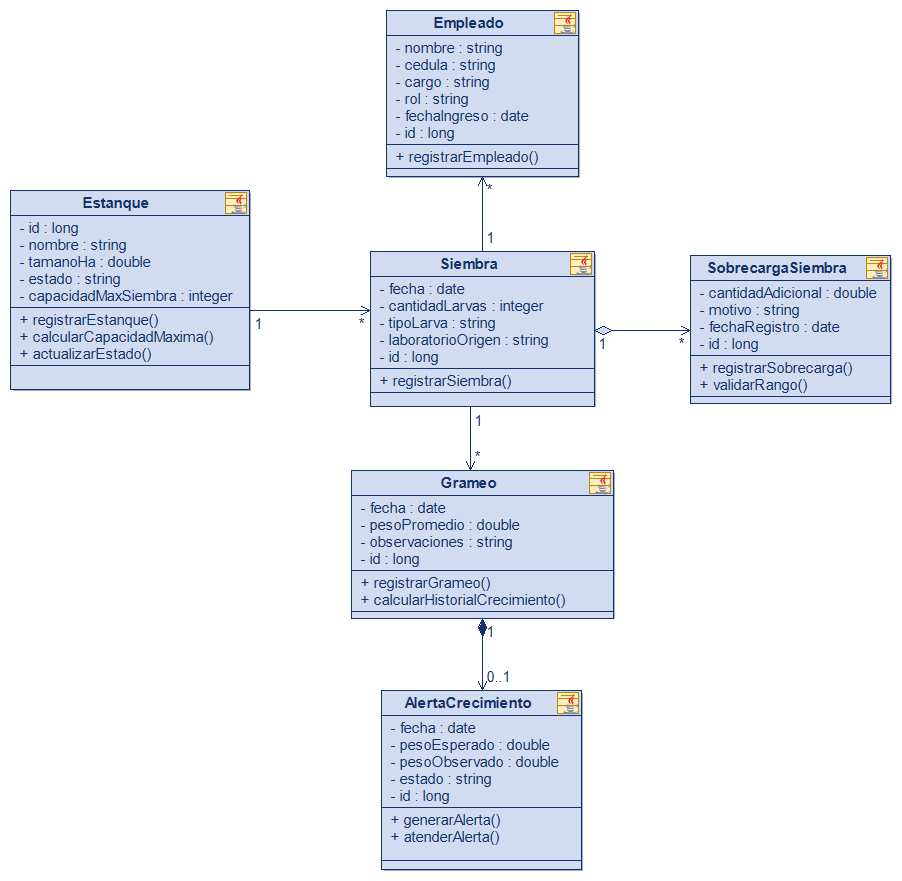
\includegraphics[width=0.6\linewidth]{figuras/ControlEstanquesSiembras Class diagram.png}
   \caption{Diagrama de clases de origen del subsistema Control de Estanques,
   Siembras y Seguimiento, exportado desde Modelio.}
  \label{fig:clases-origen}
 \end{figure}

El siguiente diagrama de clases corresponde al modelo UML desarrollado en
Modelio y utilizado como base para la generación automática de código.
Previamente se verificó la consistencia del modelo, incluyendo la correcta
nomenclatura de todas las clases, garantizando que el código generado refleje
fielmente el diseño conceptual.
\subsubsection{Relaciones}
\begin{center}
\begin{tabularx}{\linewidth}{lXl}
\toprule
\textbf{Relación} & \textbf{Multiplicidad} & \textbf{Tipo} \\
\midrule
Estanque -- Siembra & 1 a 0..* & Asociación \\
Siembra -- Empleado (responsables) & 1 a 0..* & Asociación \\
Siembra -- SobrecargaSiembra & 1 a 0..* & Agregación \\
Siembra -- Grameo & 1 a 0..* & Asociación \\
Grameo -- AlertaCrecimiento & 1 a 0..1 & Composición \\
\bottomrule
\end{tabularx}
\end{center}
Las multiplicidades de \texttt{Estanque}--\texttt{Siembra} y
\texttt{Siembra}--\texttt{Grameo} provienen directamente de la Tabla 19 del ERS;
el resto son una propuesta del equipo, a validar y ajustar dentro de Modelio si
la herramienta o el criterio del equipo sugieren un cambio.

\subsection{Diagrama de casos de uso (complementario)}
\label{sec:casos-uso}
El siguiente diagrama de casos de uso fue elaborado en Modelio 5.4 y representa las principales funcionalidades del subsistema, así como la interacción entre los actores y el sistema. Este diagrama complementa el modelo de clases al mostrar los procesos que cada tipo de usuario puede ejecutar, proporcionando una visión funcional del sistema antes de la generación automática de código.

\begin{figure}[htbp]
    \centering
    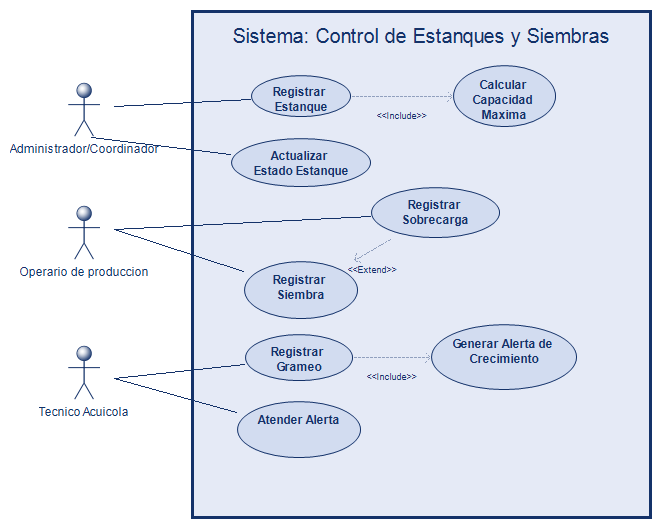
\includegraphics[width=0.62\linewidth]{figuras/project1 Use Case diagram.png}
    \caption{Diagrama de casos de uso del subsistema Control de Estanques y
    Siembras, elaborado en Modelio 5.4. Los tres actores corresponden a los
    descritos en la Sección \ref{sec:descripcion-subsistema}.}
\label{fig:casos-uso}
\end{figure}

\textbf{Nota:} Debido a que Modelio 5.4 no ofrece un elemento específico para representar el límite del sistema (Subject) en los diagramas de casos de uso, este se representó mediante un rectángulo de dibujo. Esta representación es únicamente gráfica y no altera la estructura ni el significado del modelo UML.

\subsection{Diagrama de estados (complementario)}
\label{sec:diagrama-estados}
El siguiente diagrama de estados fue elaborado en Modelio 5.4 y representa el ciclo de vida de la clase \textbf{Estanque}, mostrando las transiciones entre sus diferentes estados de acuerdo con los eventos definidos para el subsistema. Este diagrama complementa el modelo estructural al describir el comportamiento dinámico de la entidad durante su operación.

\begin{figure}[h!]
    \centering
    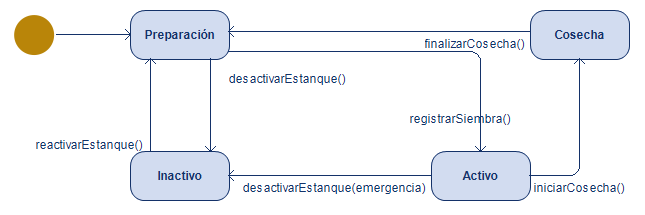
\includegraphics[width=0.65\linewidth]{figuras/State Machine State Machine diagram.png}
    \caption{Diagrama de estados de la clase \texttt{Estanque}, elaborado en
    Modelio 5.4. Las transiciones representan el ciclo de vida definido para el
    subsistema Control de Estanques y Siembras, en concordancia con el
    requisito funcional RF-04.}
    \label{fig:diagrama-estados}
\end{figure}


\subsection{Estereotipos y perfiles a aplicar}
Esta actividad genera \textbf{clases Java estándar (POJOs)}, sin persistencia:
no se usa JPA, Hibernate ni ningún ORM. Con ese alcance, el equipo creó dos
\textbf{estereotipos locales} dentro del proyecto Modelio (no importados de un
perfil externo): \verb|<<Entity>>|, aplicado a las seis clases del subsistema
para marcarlas como objetos de dominio con identidad propia, y \verb|<<Id>>|,
aplicado sobre el atributo que identifica a cada instancia dentro del modelo.
Adicionalmente, se aplicó a cada clase el estereotipo \verb|<<JavaElement>>|
requerido por el módulo Java Designer para que la clase sea reconocida como
candidata a generación de código Java.



\subsection{Validación sintáctica y semántica del modelo}
El diagrama de clases se validó dentro de Modelio mediante el panel de auditoría
del modelo (\textit{Model check}), obteniendo \textbf{0 errores y 0
advertencias} sobre las seis clases y sus relaciones (Figura
\ref{fig:validacion-modelo}). 
\begin{figure}[h!]
   \centering
   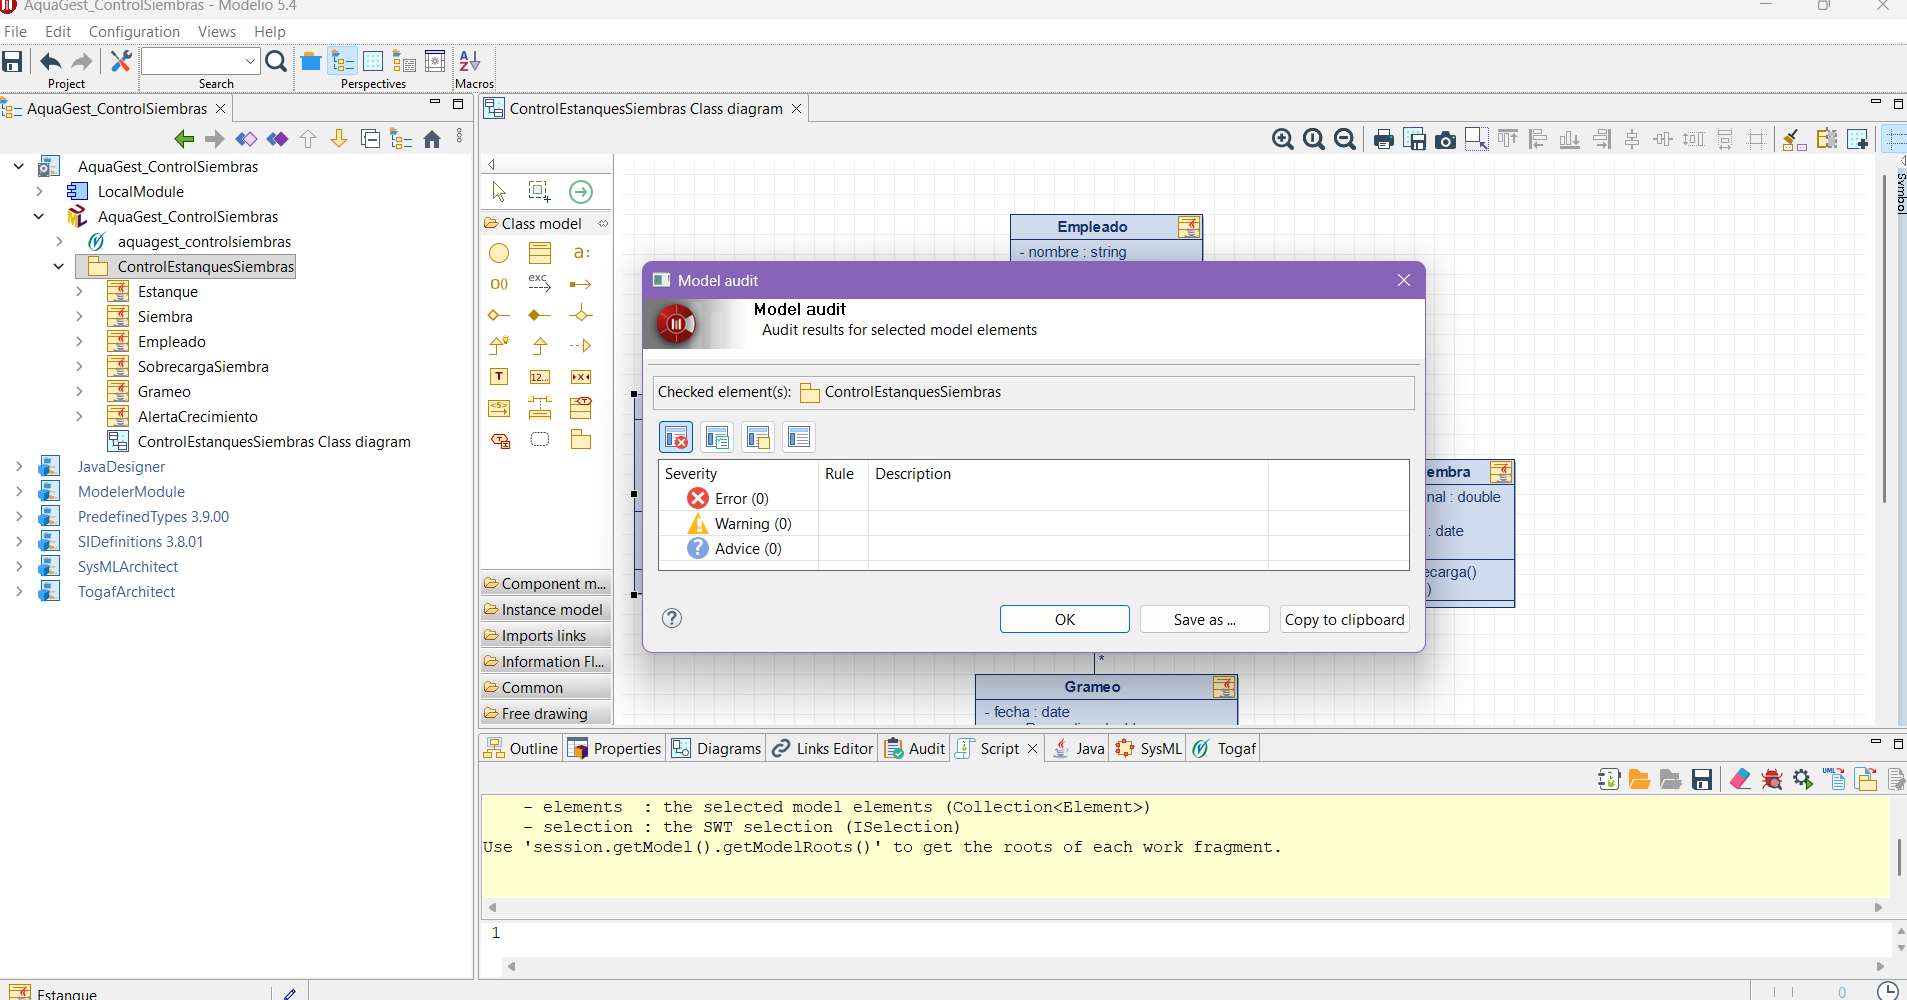
\includegraphics[width=0.8\linewidth]{figuras/Diagrama_Clases_Validacion_Sinerrores_Modelio.png}
   \caption{Panel de validación de Modelio sobre el diagrama de clases del
   subsistema: 0 errores y 0 advertencias.}
  \label{fig:validacion-modelo}
 \end{figure}
\subsection{Archivo nativo del modelo}
\label{sec:archivo-nativo}
El proyecto nativo de Modelio se exportó como archivo de proyecto
(\texttt{File > Export project}) y se subió a la carpeta \texttt{modelo/} del
repositorio de la actividad:
\begin{center}
\texttt{modelo/AquaGest\_ControlSiembras.zip}
\end{center}
Para reutilizarlo, debe importarse dentro de Modelio con
\texttt{File > Import Project...} (no descomprimirse manualmente).

% ======================= CONFIGURACIÓN DEL GENERADOR =======================
\section{Configuración del mecanismo de generación}
\label{sec:configuracion}

\subsection{Generador seleccionado}
Se utiliza el módulo de generación de código Java integrado en Modelio
(\textit{Modelio Java Designer} / \textit{Modelio SD Java}), que produce código
Java estándar directamente desde el diagrama de clases UML y mantiene la
sincronización modelo-código en modo dirigido por modelo o \textit{round-trip}
\cite{modelio_sd_java}. El alcance es la generación de \textbf{clases Java
estándar (POJOs)}, sin persistencia (no se usa JPA/Hibernate ni ningún ORM), en
coherencia con la justificación de la herramienta (Sección
\ref{sec:justificacion}).

\begin{center}
\begin{tabularx}{\linewidth}{lX}
\toprule
\textbf{Parámetro} & \textbf{Valor} \\
\midrule
Generador / módulo & Modelio Java Designer (módulo oficial) -- versión: 5.4 \\
Lenguaje objetivo & Java \\
Directorio de salida & \texttt{MODELIOJAVA} (carpeta local generada por el módulo
Java Designer; ruta completa dentro del equipo de trabajo, sin persistencia
adicional configurada) \\
Convención de nombres & \textit{PascalCase} para clases (confirmado: \texttt{
Estanque.java}, \texttt{SobrecargaSiembra.java}, etc.), \textit{camelCase} para
atributos -- observado directamente en el código generado (Sección
\ref{sec:verificacion}) \\
Política ante regeneración & El código se \textbf{sobrescribe por completo} en
cada generación: Modelio Java Designer no implementa bloques de código protegido
(\textit{protected regions}) en este módulo, por lo que no preserva
automáticamente la lógica de negocio agregada manualmente entre una generación y
la siguiente. Confirmado al ejecutar el \textit{roundtrip} controlado (Sección
\ref{sec:roundtrip}). \\
\bottomrule
\end{tabularx}
\end{center}

\subsection{Decisiones de mapeo modelo--código previstas}
\begin{center}
\begin{tabularx}{\linewidth}{>{\raggedright\arraybackslash}p{5cm}X}
\toprule
\textbf{Elemento del modelo} & \textbf{Mapeo esperado en Java} \\
\midrule
Clase \texttt{Estanque}, \texttt{Siembra}, \texttt{Grameo} & Clase Java pública
(\texttt{public class}) con el mismo nombre. \\
Atributo tipado con \texttt{double} (p. ej. \texttt{tamanoHa: double}) & Campo
privado Java (\texttt{private double tamanoHa}). La documentación del módulo
Java Designer indica que puede generar accesores \texttt{get}/\texttt{set}
automáticamente, aunque no se observaron en las clases inspeccionadas (Sección
\ref{sec:verificacion}). Si en la verificación se detecta que algún cálculo
requiere precisión exacta (p. ej. costos), se ajustará manualmente a
\texttt{BigDecimal} tras la generación. \\
Asociación Estanque--Siembra (1 a 0..*) & Colección tipada en el lado ``0..*''
(\texttt{private List<Siembra> siembras}) y referencia simple en el lado ``1''. \\
Operación (p. ej. \texttt{calcularCapacidadMaxima()}) & Firma de método Java
generada desde la operación UML; el cuerpo del método debe completarse manualmente
tras la generación, ya que la lógica de negocio no forma parte del modelo
estructural. \\
\bottomrule
\end{tabularx}
\end{center}

Estas decisiones de mapeo son la interpretación esperada según el comportamiento
documentado del generador de Modelio; deberán confirmarse o corregirse con la
evidencia real observada en la Fase 4 del procedimiento, y las eventuales
correcciones deben incorporarse a esta tabla.

\subsection{Archivos de configuración o plantilla}
Para esta actividad \textbf{no se editó ni personalizó} la plantilla estándar
del módulo Java Designer: se utilizó el generador tal como lo distribuye
Modelio, sin modificar sus reglas internas de mapeo modelo--código. Por esta
razón, la carpeta \texttt{plantillas/} del repositorio no contiene archivos de
plantilla personalizados. Si en una futura iteración del PFC se decide
personalizar la plantilla (por ejemplo, para incorporar anotaciones JPA), esta
subsección deberá actualizarse.

% ======================= PROCESO DE GENERACIÓN =======================
\section{Proceso de generación}
\label{sec:proceso-generacion}

Esta sección documenta la ejecución de la generación de código y su verificación
inicial, y debe completarse íntegramente con evidencia tomada durante la
demostración en vivo. Se mantiene aquí la estructura prevista de los tres
subapartados para que el equipo únicamente deba insertar, en su momento, las
capturas y los datos reales observados.

\subsection{Invocación del generador}
Captura de pantalla de la invocación del generador dentro de
Modelio (menú de generación de código sobre el paquete/clases del subsistema
Control de Estanques y Siembras). Modelio Java Designer no despliega una consola
de log: al invocar \textit{Generate}, el proceso corre y finaliza sin mostrar
ventana ni mensaje de salida; la confirmación de éxito se obtiene directamente del
árbol de archivos resultante (ver subapartado siguiente).
 \begin{figure}[h!]
   \centering
   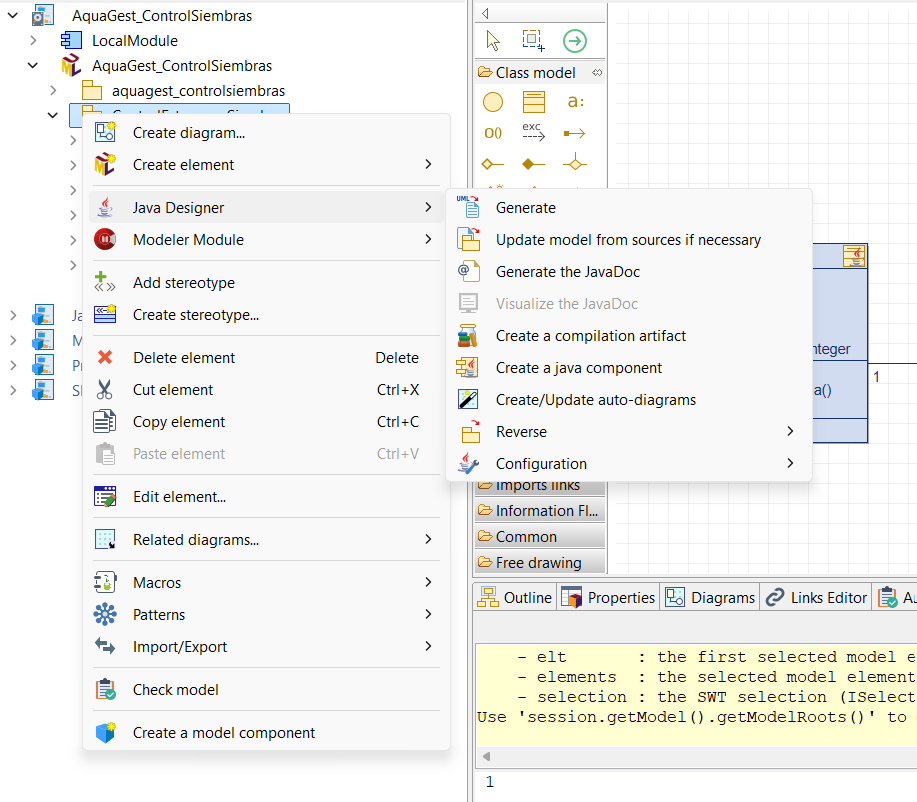
\includegraphics[width=0.62\linewidth]{figuras/generador_codigo_java_designer.png}
   \caption{Invocación del generador de código en Modelio.}
 \end{figure}

\subsection{Árbol del proyecto generado}
La generación produjo seis archivos Java, uno por cada clase del subsistema, en la
carpeta de salida \texttt{MODELIOJAVA} (Figura \ref{fig:archivos-generados}):
\texttt{Estanque.java}, \texttt{Siembra.java}, \texttt{SobrecargaSiembra.java},
\texttt{Grameo.java}, \texttt{AlertaCrecimiento.java} y \texttt{Empleado.java}.
 \begin{figure}[h!]
   \centering
   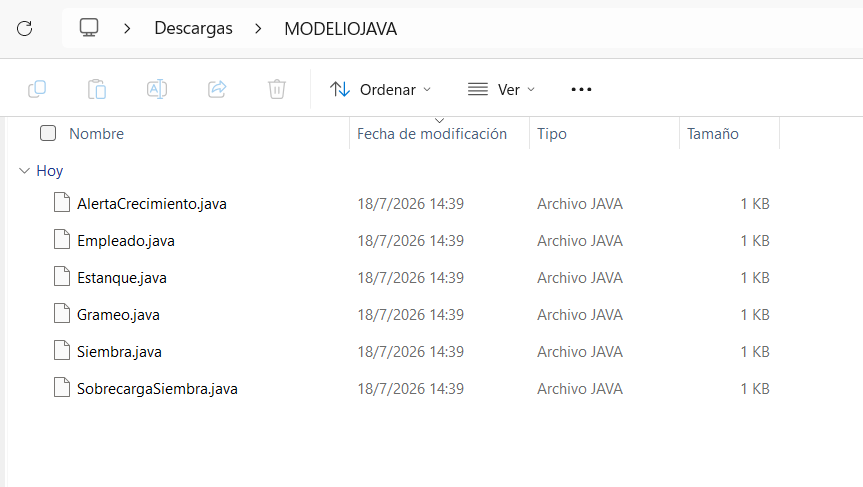
\includegraphics[width=0.68\linewidth]{figuras/archivos_generados.png}
   \caption{Árbol de archivos \texttt{.java} generados por Modelio Java Designer
   en la carpeta \texttt{MODELIOJAVA}.}
   \label{fig:archivos-generados}
 \end{figure}

\subsection{Tiempos de generación}
Los seis archivos generados muestran la misma marca de tiempo de modificación (\texttt{18/7/2026 14:39}) y un tamaño uniforme de 1 KB cada uno (Figura \ref{fig:archivos-generados}), lo que evidencia que la generación del código se realizó de forma prácticamente instantánea para las seis clases del subsistema.


% ======================= VERIFICACIÓN DEL CÓDIGO =======================
\section{Verificación del código generado}
\label{sec:verificacion}

\subsection{Evidencia de compilación y ejecución}

El código generado se abrió en \textbf{IntelliJ IDEA}, dentro del proyecto
\texttt{MODELIOJAVA}. El inspector estático del IDE no reporta problemas sobre la
clase \texttt{AlertaCrecimiento.java} (``No problems in AlertaCrecimiento.java'',
Figura \ref{fig:codigo-intellij}), lo que confirma que ese archivo es
sintácticamente válido.

\begin{figure}[h!]
   \centering
   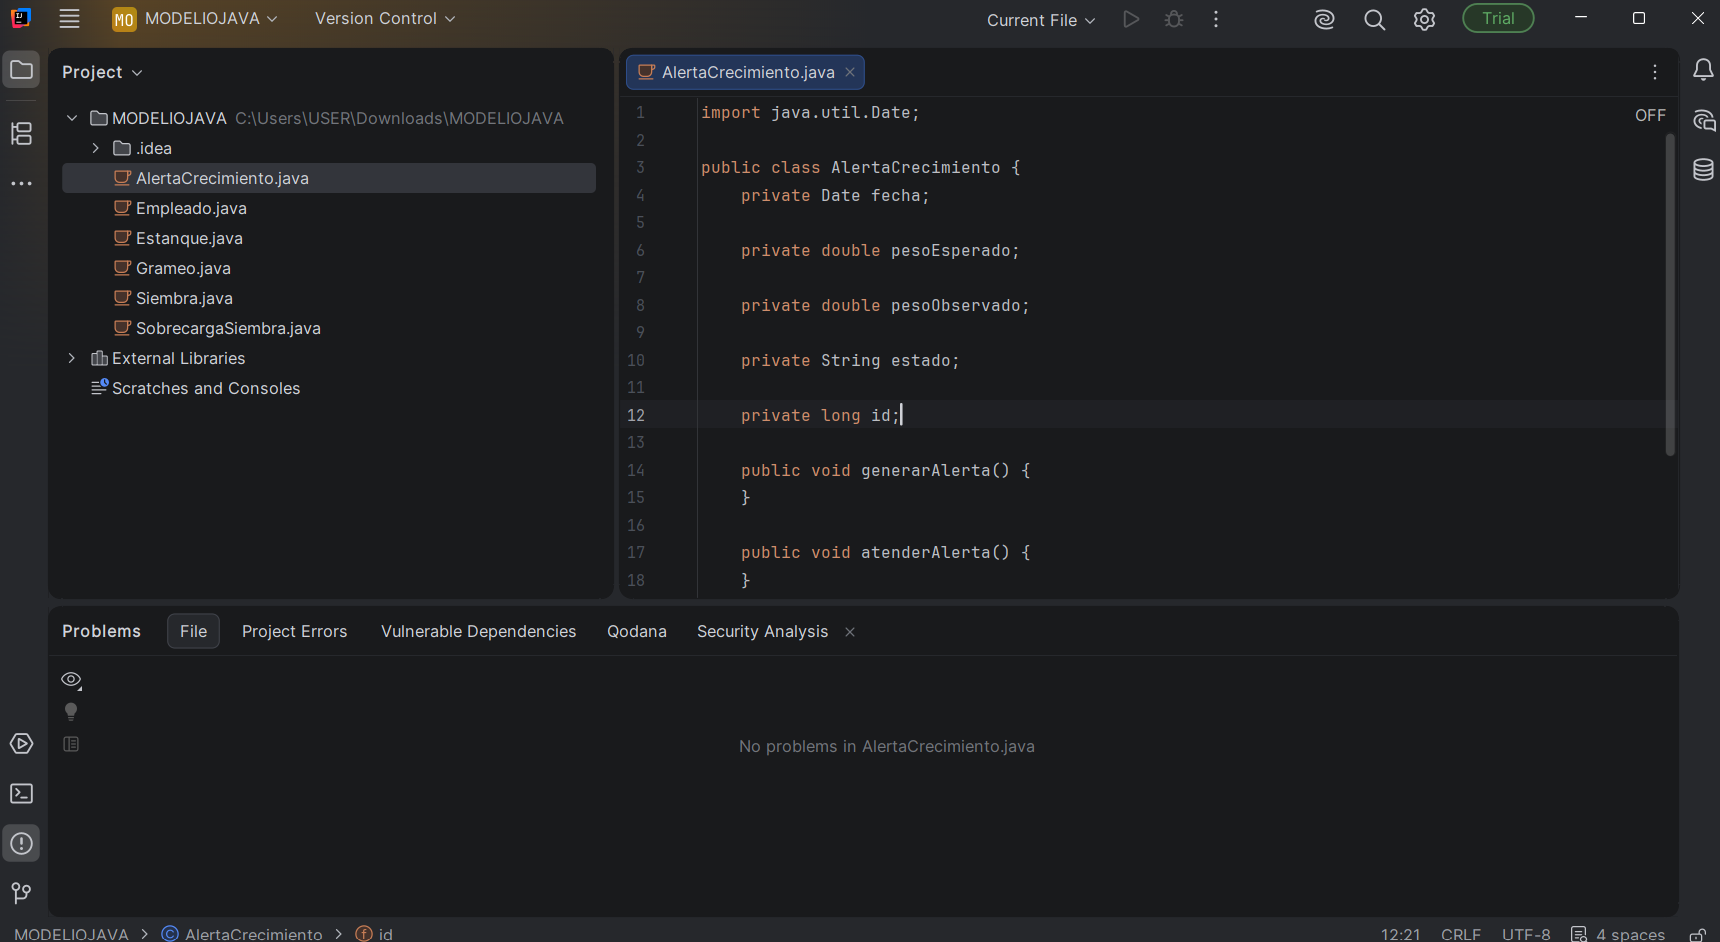
\includegraphics[width=0.68\linewidth]{figuras/codigo_generado_en_IntelliJ.png}
  \caption{Clase \texttt{AlertaCrecimiento.java} generada, abierta en IntelliJ IDEA
  sin problemas reportados por el inspector estático.}
  \label{fig:codigo-intellij}
 \end{figure}

\subsection{Correspondencia modelo $\rightarrow$ código}
\label{sec:correspondencia}
La existencia de los seis archivos \texttt{.java} está confirmada por el árbol de
archivos generado (Figura \ref{fig:archivos-generados}, Sección
\ref{sec:proceso-generacion}). El contenido detallado se inspeccionó
directamente para dos clases: \texttt{AlertaCrecimiento.java} (Figura
\ref{fig:codigo-intellij}) y \texttt{Siembra.java}, esta última visible en las
capturas del \textit{roundtrip} (Figuras \ref{fig:roundtrip-antes} y
\ref{fig:roundtrip-regeneracion}, Sección \ref{sec:roundtrip}). Para las tres
clases restantes (\texttt{Estanque}, \texttt{Empleado}, \texttt{Grameo},
\texttt{SobrecargaSiembra}) aún debe abrirse cada archivo y contrastarlo con
esta tabla.

\begin{center}
\begin{tabularx}{\linewidth}{>{\raggedright\arraybackslash}p{3.7cm}XX}
\toprule
\textbf{Elemento del modelo} & \textbf{Artefacto generado esperado} &
\textbf{Verificado} \\
\midrule
Clase \texttt{Estanque} & Archivo \texttt{Estanque.java} & Sí (archivo existe) \\
Clase \texttt{Siembra} & Archivo \texttt{Siembra.java} & \textbf{Sí, verificado
en código}: campos \texttt{fecha}, \texttt{cantidadLarvas}, \texttt{tipoLarva},
\texttt{laboratorioOrigen}, \texttt{id} (autogenerado). \\
Clase \texttt{Grameo} & Archivo \texttt{Grameo.java} & Sí (archivo existe) \\
Clase \texttt{Empleado} & Archivo \texttt{Empleado.java} & Sí (archivo existe) \\
Clase \texttt{SobrecargaSiembra} & Archivo \texttt{SobrecargaSiembra.java} &
Sí (archivo existe) \\
Clase \texttt{AlertaCrecimiento} & Archivo \texttt{AlertaCrecimiento.java} &
\textbf{Sí, verificado en código}: campos \texttt{fecha}, \texttt{pesoEsperado},
\texttt{pesoObservado}, \texttt{estado}, \texttt{id} y métodos
\texttt{generarAlerta()}, \texttt{atenderAlerta()} coinciden 1:1 con el modelo. \\
Atributo \texttt{Estanque.tamanoHa} & Campo \texttt{tamanoHa} + accesores &
Pendiente (falta abrir \texttt{Estanque.java}) \\
Asociación Estanque--Siembra & Colección \texttt{List<Siembra>} en
\texttt{Estanque.java} & Pendiente -- \texttt{Siembra.java} no contiene una
referencia de vuelta a \texttt{Estanque} (coherente con una asociación
unidireccional 1 a 0..*), pero el lado ``1'' (\texttt{Estanque.java}) no ha
sido inspeccionado. \\
Asociación Siembra--Grameo & Colección \texttt{List<Grameo>} en
\texttt{Siembra.java} & \textbf{Sí, verificado en código}: se generó
\texttt{public List<Grameo>} en \texttt{Siembra.java}. \\
Asociación Siembra--Empleado (responsables) & Colección \texttt{List<Empleado>}
en \texttt{Siembra.java} & \textbf{Sí, verificado en código}: se generó
\texttt{public List<Empleado>} en \texttt{Siembra.java}, coherente con la
navegabilidad Siembra $\rightarrow$ Empleado y la multiplicidad 1 a 0..* del
modelo (una siembra puede tener más de un empleado responsable). \\
Agregación Siembra--SobrecargaSiembra & Colección
\texttt{List<SobrecargaSiembra>} en \texttt{Siembra.java} & \textbf{Sí,
verificado en código}: se generó \texttt{public List<SobrecargaSiembra>} en
\texttt{Siembra.java}. \\
Composición Grameo--AlertaCrecimiento & Referencia \texttt{AlertaCrecimiento} en
\texttt{Grameo.java} & Pendiente (falta abrir \texttt{Grameo.java}) \\
Operación \texttt{registrarSiembra()} & Firma de método en \texttt{Siembra.java} &
\textbf{Sí, verificado en código}: existe como \texttt{public void
registrarSiembra()} con cuerpo vacío (ver Sección \ref{sec:roundtrip} para la
prueba de sobrescritura tras regenerar). \\
\bottomrule
\end{tabularx}
\end{center}

\newpage
\subsection{Limitaciones observadas del generador}
\label{sec:limitaciones}
A partir de la revisión directa de \texttt{AlertaCrecimiento.java} y
\texttt{Siembra.java} se verificó que el generador produce correctamente la
estructura básica de una clase (atributos tipados, identificador autogenerado y
firmas de operación) a partir del modelo UML. Los cuerpos de las operaciones
(\texttt{generarAlerta()}, \texttt{atenderAlerta()}, \texttt{registrarSiembra()})
se generaron \textbf{vacíos}: la implementación de la lógica de negocio debe
desarrollarse manualmente. Este comportamiento es consistente con el
funcionamiento esperado de un generador de código estructural, cuyo objetivo es
producir la estructura del sistema y no la implementación de sus reglas de
negocio.

Se confirmó también que la asociación Siembra--Empleado se refleja
correctamente como \texttt{public List<Empleado>} en \texttt{Siembra.java},
coherente con la navegabilidad Siembra $\rightarrow$ Empleado y la
multiplicidad 1 a 0..* definida en el modelo (Sección
\ref{sec:diagrama-clases}): una siembra puede tener más de un empleado
responsable.

Finalmente, las validaciones propias de los requisitos funcionales, como la
verificación de que la cantidad de larvas no supere la capacidad máxima de
siembra establecida por el requisito funcional RF-05, no son implementadas
automáticamente por Modelio y deben incorporarse manualmente durante la etapa de
desarrollo.


% ======================= CIERRE DEL CICLO (ROUNDTRIP) =======================
\section{Cierre del ciclo (\textit{roundtrip} controlado)}
\label{sec:roundtrip}

\subsection{Cambio propuesto en el modelo}
Como cambio no trivial para evidenciar el cierre del ciclo MDD, se propone agregar
un nuevo atributo a la clase \texttt{Siembra}: \texttt{porcentajeSupervivenciaInicial:
double}, que registra el porcentaje estimado de supervivencia de las larvas al
momento de la siembra (dato mencionado como relevante en el acta de entrevista con el
Técnico Acuícola, Apéndice B.3 del ERS de AquaGest, aunque todavía no formalizado
como RF independiente). Este cambio es representativo porque:
\begin{itemize}[leftmargin=1.5em]
    \item No es un cambio trivial de tipo tipográfico, sino la incorporación de un
    dato de negocio nuevo.
    \item Debe reflejarse tanto en el modelo (nuevo atributo con su tipo) como en el
    código generado (nuevo campo).
    \item Permite verificar si el módulo de generación preserva el código
    manualmente añadido en los métodos ya completados en la Fase 5, o si lo
    sobrescribe.
\end{itemize}
\newpage
\subsection{Evidencia antes/después}
\begin{itemize}[leftmargin=1.5em]
    \item Captura del modelo \textbf{antes} del cambio (diagrama de clases con
    \texttt{Siembra} en su versión original).
    \item Captura del modelo \textbf{después} del cambio, con el nuevo atributo agregado (observaciones).

\end{itemize}

% Pendiente: capturas antes/después del modelo y del código.
 \begin{figure}[h!]
   \centering
   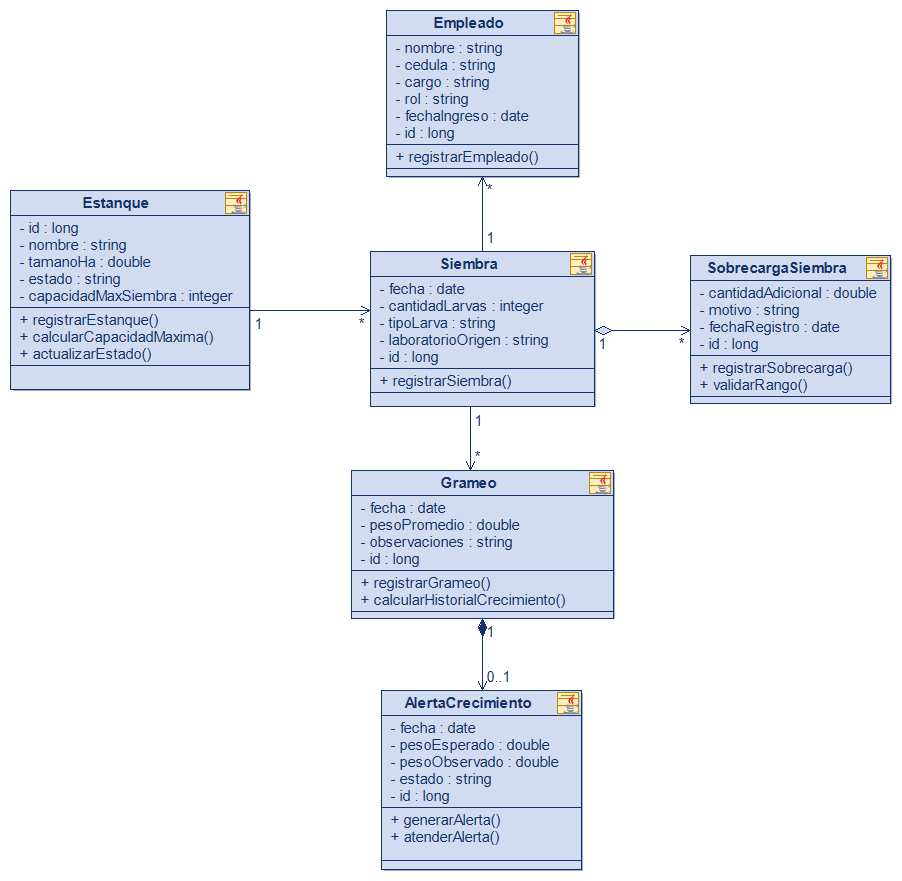
\includegraphics[width=0.48\linewidth]{figuras/ControlEstanquesSiembras Class diagram.png}
   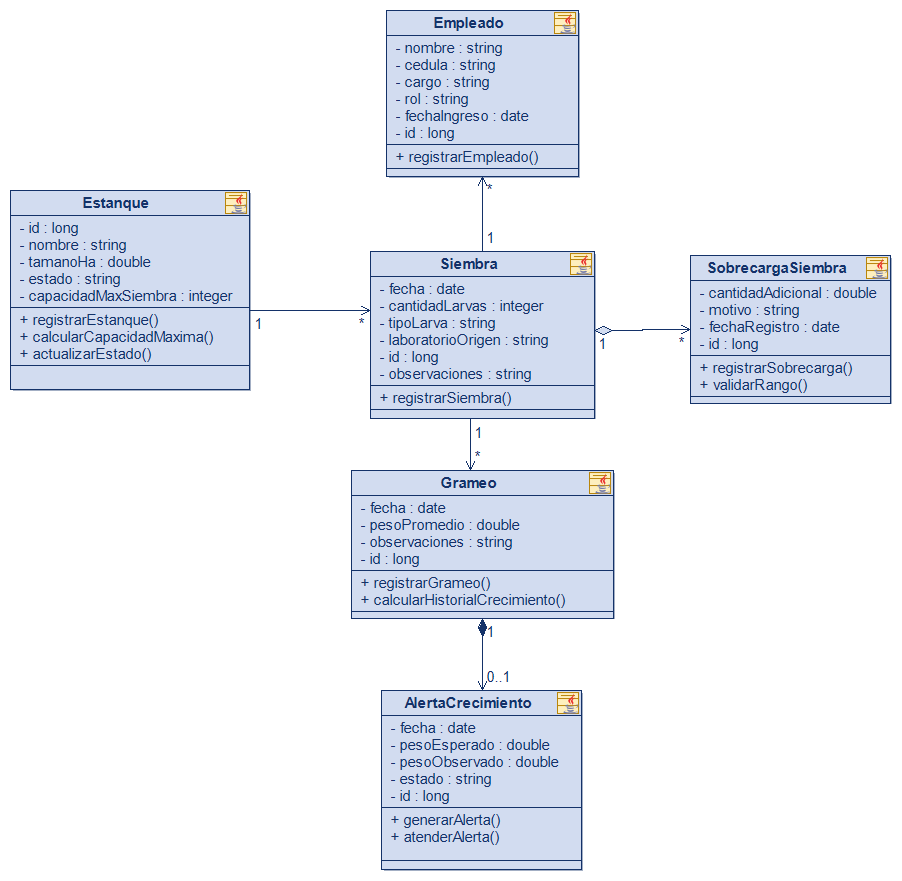
\includegraphics[width=0.48\linewidth]{figuras/Diagrama_despues.png}
   \caption{Modelo antes y después del cambio en \texttt{Siembra}.}
 \end{figure}

 \begin{itemize}[leftmargin=1.5em]
    \item Captura del código generado \textbf{antes} de la regeneración.
    \item Captura del código generado \textbf{después} de la regeneración, mostrando
    el nuevo campo.
\end{itemize}

 \begin{figure}[h!]
  \centering
   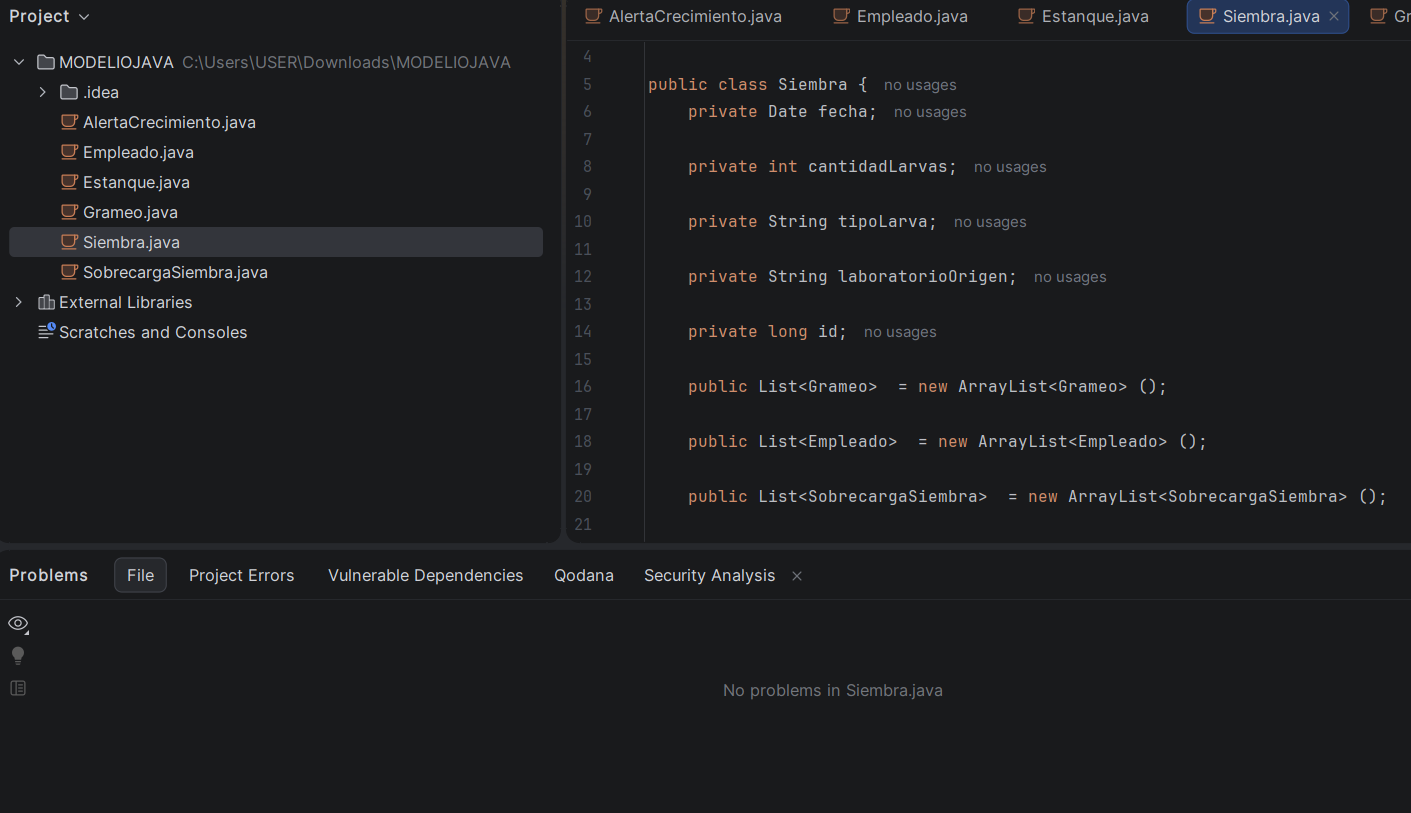
\includegraphics[width=0.48\linewidth]{figuras/antes_codigo_clase.png}
   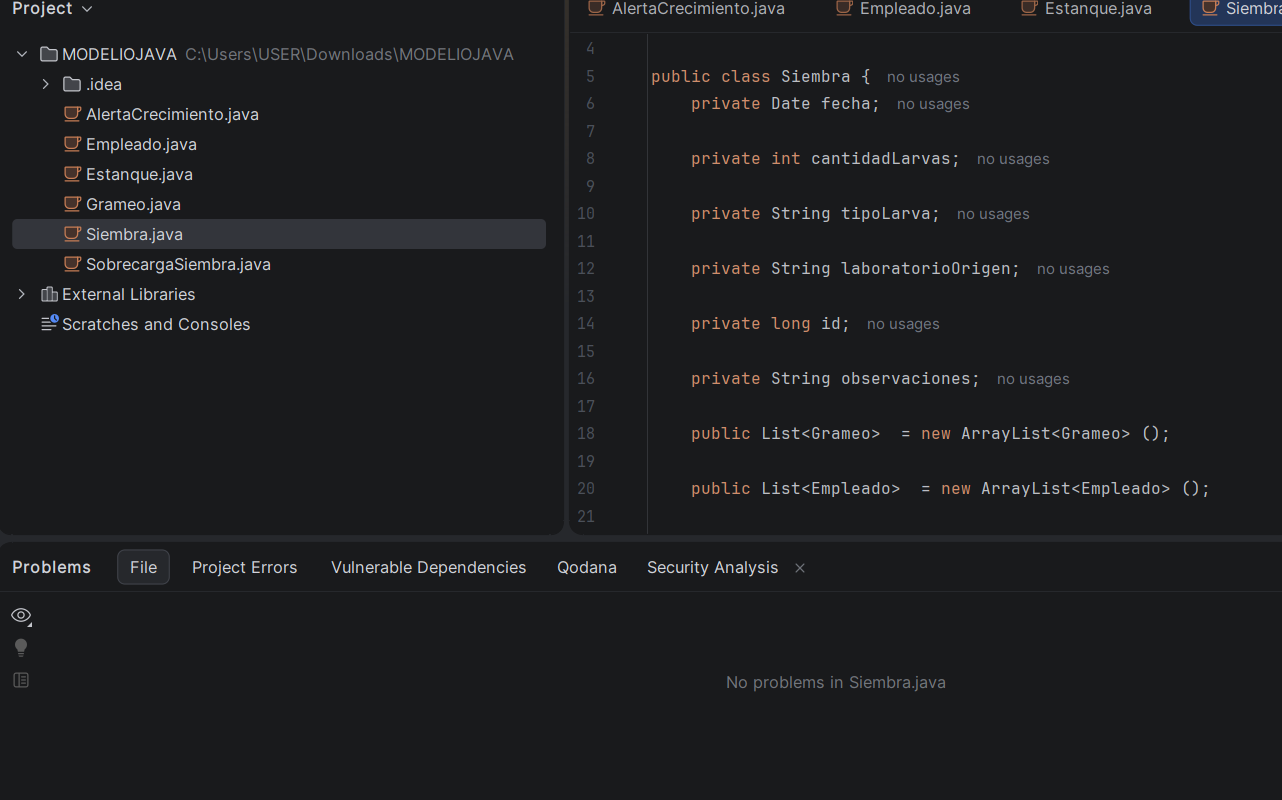
\includegraphics[width=0.48\linewidth]{figuras/despues_codigo_clase.png}
   \caption{Código Java de \texttt{Siembra} generado por Modelio, antes y
   después de la regeneración con el nuevo atributo
   \texttt{porcentajeSupervivenciaInicial} agregado en el modelo.}
   \label{fig:roundtrip-antes}
 \end{figure}

\subsection{Manejo de bloques protegidos}

Modelio Java Designer, en el modo de generación utilizado en esta actividad, \textbf{no implementa bloques de código protegido} (\textit{protected regions}) que preserven automáticamente la lógica de negocio agregada manualmente entre una generación y la siguiente. Como se documentó en la Sección \ref{sec:configuracion} (``Política ante regeneración''), cada ejecución del generador \textbf{sobrescribe por completo} el archivo \texttt{.java} correspondiente con el contenido derivado del modelo.

En consecuencia, para evitar la pérdida de trabajo manual al regenerar el código, se recomienda adoptar una de las siguientes estrategias:

\begin{enumerate}[leftmargin=1.5em]
    \item \textbf{Respaldo manual:} copiar fuera del árbol \texttt{MODELIOJAVA} la lógica de negocio implementada antes de regenerar el código y reincorporarla posteriormente mediante copia/pegado o utilizando un sistema de control de versiones.

    \item \textbf{Separación en clases de servicio (recomendada):} trasladar la lógica de negocio a clases de servicio o utilitarias independientes, fuera del árbol de clases de dominio generado por Modelio, de modo que la regeneración de \texttt{Estanque}, \texttt{Siembra}, \texttt{Grameo}, \texttt{AlertaCrecimiento}, \texttt{SobrecargaSiembra} y \texttt{Empleado} no afecte dicha lógica. Esta estrategia resulta adecuada para el desarrollo posterior del PFC y es coherente con la arquitectura cliente-servidor por capas definida en la restricción RST-05 de la ERS.
\end{enumerate}

\begin{figure}[h!]
    \centering
    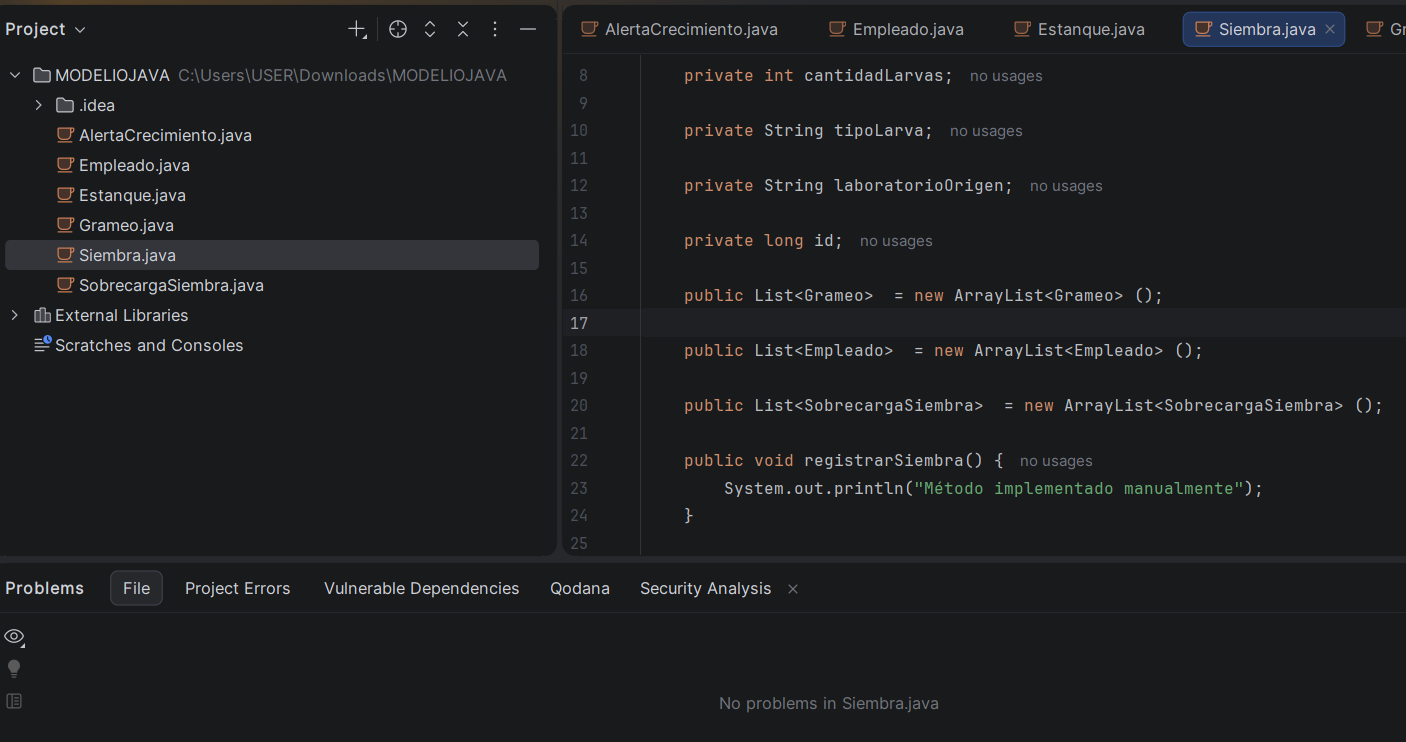
\includegraphics[width=0.48\linewidth]{figuras/antes_metodo_modificado.png}
    \hfill
    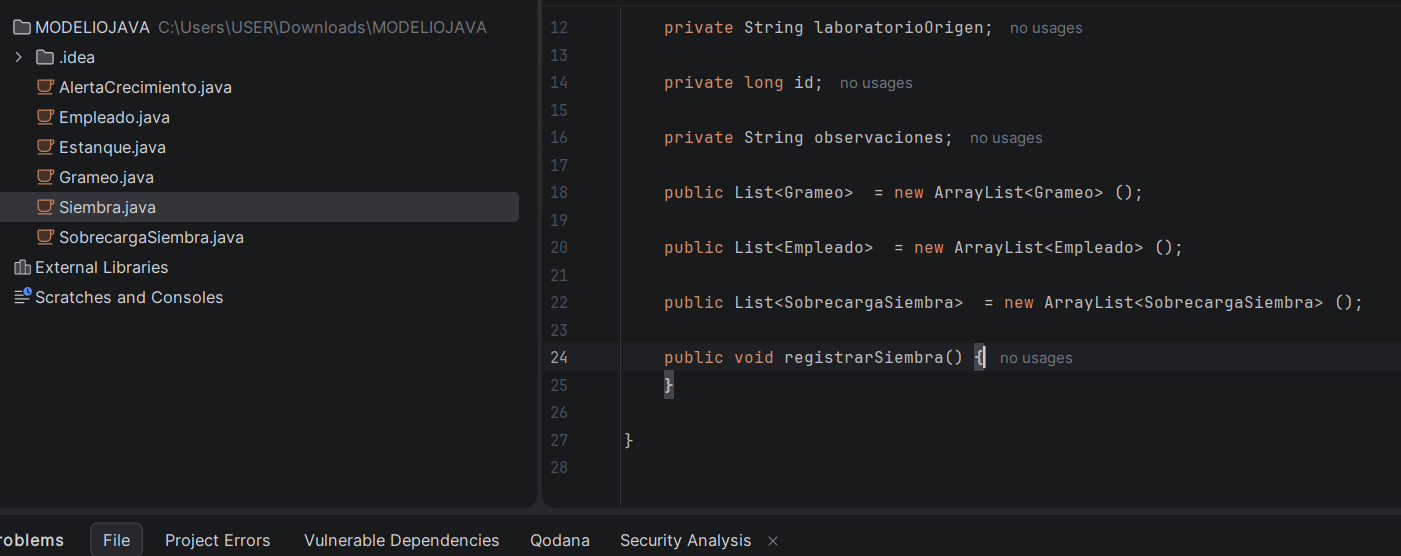
\includegraphics[width=0.48\linewidth]{figuras/despues_regeneraion.png}
    \caption{Código generado antes (con una modificación manual en el método \texttt{registrarSiembra()}) y después de la regeneración desde Modelio. Se observa que la modificación manual fue reemplazada por el código generado automáticamente.}
    \label{fig:roundtrip-regeneracion}
\end{figure}

La Figura \ref{fig:roundtrip-regeneracion} evidencia que, tras modificar manualmente el método \texttt{registrarSiembra()} y ejecutar nuevamente la generación de código, los cambios realizados fueron sobrescritos. Esto confirma que Modelio Java Designer, con la configuración utilizada en esta práctica, no preserva automáticamente las modificaciones manuales mediante bloques protegidos, por lo que es necesario respaldar el código o separar la lógica de negocio en clases no generadas antes de regenerar el proyecto.

\subsection{Trazabilidad modelo $\rightarrow$ código tras el cambio}

A pesar de que la regeneración sobrescribe las modificaciones manuales realizadas en los archivos \texttt{.java}, la trazabilidad entre el modelo UML y el código generado se mantuvo durante la práctica. Después de realizar modificaciones en el modelo de Modelio y ejecutar nuevamente la generación de código, se verificó que los cambios definidos en el modelo fueron reflejados correctamente en los archivos Java correspondientes. Asimismo, se comprobó que la correspondencia entre clases, atributos, operaciones y relaciones se conservó tras la regeneración. La Tabla presentada en la Sección \ref{sec:correspondencia} resume la verificación de dicha trazabilidad.
\newpage
% ======================= REPARTO DEL TRABAJO =======================
\section{Reparto del trabajo por integrante}
\label{sec:reparto}

La distribución de tareas para esta actividad corresponde al equipo asignado a la
exposición-demostración MDD, integrado por tres miembros.

\begin{center}
\begin{tabularx}{\linewidth}{p{3cm}XX}
\toprule
\textbf{Integrante} & \textbf{Rol en la actividad MDD} & \textbf{Tarea concreta
asignada} \\
\midrule
Amagua Sacon Robyn Willian & Coordinación general, justificación de la herramienta
& Coordina al equipo y los tiempos de la exposición, redacta
la justificación de Modelio frente a las restricciones del PFC (Sección
\ref{sec:justificacion}), y estructura/mantiene este documento evidencia en LaTeX. \\
Crespo Espinoza Kleber Obed & Modelado UML en Modelio y documentación LaTeX &
Construye los diagramas de clases, casos de uso y estados dentro de Modelio
(Sección \ref{sec:modelo-uml}), aplica estereotipos y ejecuta la validación
sintáctica/semántica del modelo. \\
Rizzo Velez Edson Nagib & Configuración del generador, ejecución de la generación,
verificación de código y cierre del ciclo & Configura los parámetros del módulo de
generación (Sección \ref{sec:configuracion}), ejecuta el proceso de generación
(Sección \ref{sec:proceso-generacion}), verifica la compilación/ejecución del
código generado (Sección \ref{sec:verificacion}) y ejecuta el \textit{roundtrip}
controlado documentado en la Sección \ref{sec:roundtrip}. \\
\bottomrule
\end{tabularx}
\end{center}

\subsection{Commits diferenciados por integrante}
Se registra a continuación la lista de commits atribuibles a cada integrante.



\begin{tabularx}{\textwidth}{
>{\raggedright\arraybackslash}p{0.14\textwidth}
>{\raggedright\arraybackslash}X
>{\raggedright\arraybackslash}p{0.26\textwidth}
}
\toprule
\textbf{Integrante} & \textbf{Contribución (mensaje del commit)} & \textbf{URL del commit} \\
\midrule

% --- Amagua Sacon Robyn Willian ---
Amagua Sacon Robyn Willian &
\begin{itemize}[leftmargin=*,nosep,itemsep=2pt]
    \item \textbf{Add files via upload.} Documento en LaTeX que reúne la evidencia del trabajo realizado con Modelio para generar código a partir de diagramas UML en el proyecto AquaGest.
    \item \textbf{Add files via upload.} Archivo de bibliografía en formato BibTeX con las referencias utilizadas en el informe.
    \item \textbf{Código generado de la clase Siembra.}
    \item \textbf{Código generado de la clase SobrecargaSiembra.}
    \item \textbf{Diapositivas de Exposición de la herramienta Modelio.}
\end{itemize} &
\begin{itemize}[leftmargin=*,nosep,itemsep=2pt]
    \item \href{https://github.com/erizzov-boop/PFC-AquaGest-MDD-Equipo_D-/commit/733bd48c5aa8d644316a9d1d99432ee01166b8e6}{733bd48}
    \item \href{https://github.com/erizzov-boop/PFC-AquaGest-MDD-Equipo_D-/commit/6b44903f906eb46bc1c1df2e47a9f55b36ffd855}{6b44903}
    \item \href{https://github.com/erizzov-boop/PFC-AquaGest-MDD-Equipo_D-/commit/05ddb819f208bbfa3a87db02157e54e234072dba}{05ddb81}
    \item \href{https://github.com/erizzov-boop/PFC-AquaGest-MDD-Equipo_D-/commit/b48b2c76bb84dee90b6d2e8c74deee80e02218c3}{b48b2c7}
    \item \href{https://github.com/erizzov-boop/PFC-AquaGest-MDD-Equipo_D-/commit/11853614a42dd13a97bd3a23646500306fac05f4}{1185361}
\end{itemize} \\

\midrule

% --- Crespo Espinoza Kleber Obed ---
Crespo Espinoza Kleber Obed &
\begin{itemize}[leftmargin=*,nosep,itemsep=2pt]
    \item \textbf{Agregar secciones 3, 4 y 5 del informe.} Se incorporaron las subsecciones: 3. Descripción del subsistema del PFC modelado (contexto, actores, subsistema seleccionado, requisitos funcionales cubiertos, alcance del módulo); 4. Modelo UML de origen (origen de los datos, clases, diagrama de clases con sus relaciones, diagrama de casos de uso, diagrama de estados, estereotipos y perfiles, validación sintáctica y semántica, archivo nativo); 5. Configuración del mecanismo de generación (generador seleccionado, decisiones de mapeo modelo--código, archivos de configuración o plantilla).
    \item \textbf{Código generado de clase Estanque.}
    \item \textbf{Código generado de clase Grameo.}
    \item \textbf{Agrega proyecto exportado desde Modelio.}
    \item \textbf{Agrega conclusiones.} Se añaden las subsecciones 10.1 Valor del ciclo MDD para el PFC AquaGest; 10.2 Aprendizajes obtenidos; 10.3 Limitaciones.
    
\end{itemize} &
\begin{itemize}[leftmargin=*,nosep,itemsep=2pt]
    \item \href{https://github.com/erizzov-boop/PFC-AquaGest-MDD-Equipo_D-/commit/a4a0bf6ff8b658e6f0d7d01a9128421c529fd1d2}{a4a0bf6}
    \item \href{https://github.com/erizzov-boop/PFC-AquaGest-MDD-Equipo_D-/commit/fc1e8f6ff10e38bdcaa99779135dcf219c0f6b7d}{fc1e8f6}
    \item \href{https://github.com/erizzov-boop/PFC-AquaGest-MDD-Equipo_D-/commit/ade5550524638a1ac49a4ffe7a938a1661368262}{ade5550}
    \item \href{https://github.com/erizzov-boop/PFC-AquaGest-MDD-Equipo_D-/commit/b6ac964680bba44dc6c075c1e8dca8900d95ab84}{b6ac964}
    \item \href{https://github.com/erizzov-boop/PFC-AquaGest-MDD-Equipo_D-/commit/34845d35ca3f3a1a1ebe81cd3643d88c017e6e39}{34845d3}
\end{itemize} \\

\midrule

% --- Rizzo Vélez Edson Nagib ---
Rizzo Vélez Edson Nagib &
\begin{itemize}[leftmargin=*,nosep,itemsep=2pt]
    \item \textbf{Agregar sección 6, 7, 8 y 9.} Junto con las secciones adjuntadas también se agregaron las figuras usadas respectivamente en estas.
    \item \textbf{Código generado de la clase AlertaCrecimiento.}
    \item \textbf{Código generado de la clase Empleado.}
    \item \textbf{Update readme.} Se actualiza el archivo \texttt{modelo/perfiles/readme} indicando que no se utilizaron perfiles.
    \item \textbf{Agregar video demostrativo.} Se añade el archivo \texttt{evidencias/video-demo.mp4}.
    \item \textbf{Update readme.}
    \item \textbf{Update README.md.}
    \item \textbf{Update readme no se usaron plantillas.} Descripción del uso de plantillas.
\end{itemize} &
\begin{itemize}[leftmargin=*,nosep,itemsep=2pt]
    \item \href{https://github.com/erizzov-boop/PFC-AquaGest-MDD-Equipo_D-/commit/4004abddd626857ddcc8d418f9c7ef1a36a638d6}{4004abd}
    \item \href{https://github.com/erizzov-boop/PFC-AquaGest-MDD-Equipo_D-/commit/d038efa7f5951c64e846ba8c8aea5a2c17b7d7ea}{d038efa}
    \item \href{https://github.com/erizzov-boop/PFC-AquaGest-MDD-Equipo_D-/commit/5f2600cfd15a637b67cd662eee6f198a3014f253}{5f2600c}
    \item \href{https://github.com/erizzov-boop/PFC-AquaGest-MDD-Equipo_D-/commit/6cd895bc7a4abd72daffeaf900c7b995d1aa9fe1}{6cd895b}
    \item \href{https://github.com/erizzov-boop/PFC-AquaGest-MDD-Equipo_D-/commit/714de4a616b28aa90208116057237273ccc0f9f8}{714de4a}
    \item \href{https://github.com/erizzov-boop/PFC-AquaGest-MDD-Equipo_D-/commit/1c8bac3e1705e6a99e8a3254a9cbc985ae59c9e1}{1c8bac3}
    \item \href{https://github.com/erizzov-boop/PFC-AquaGest-MDD-Equipo_D-/commit/f52e82325b3fcdbb94d24648461c7dce836de557}{f52e823}
    \item \href{https://github.com/erizzov-boop/PFC-AquaGest-MDD-Equipo_D-/commit/dbbd3ab99325e0459107ef74bf4304efb6380663}{dbbd3ab}
\end{itemize} \\

\bottomrule
\end{tabularx}







% ======================= CONCLUSIONES =======================
\section{Conclusiones}
\label{sec:conclusiones}

\subsection{Valor del ciclo MDD para el PFC AquaGest}
La aplicación del ciclo MDD con Modelio sobre el subsistema de Control de
Estanques, Siembras y Seguimiento permite verificar, de forma concreta, que el
modelo de dominio (clases \texttt{Estanque}, \texttt{Siembra}, \texttt{Empleado},
\texttt{SobrecargaSiembra}, \texttt{Grameo} y \texttt{AlertaCrecimiento}, con
base en los RF-01 a RF-08 y RF-17 ya formalizados y validados con el stakeholder
de la Compañía Biofina) es suficientemente preciso como para derivar de él una
base de código estructural, reduciendo el riesgo de que la implementación
posterior del PFC se desvíe de esos requisitos. La verificación directa del
código generado (Sección \ref{sec:correspondencia}) confirmó que Modelio Java
Designer respeta fielmente la navegabilidad y la multiplicidad definidas en el
modelo, lo que refuerza la confiabilidad del ciclo MDD como punto de partida
para el desarrollo posterior del PFC, sin eximir de completar manualmente la
lógica de negocio (Sección \ref{sec:limitaciones}).

\subsection{Aprendizajes obtenidos}

La ejecución de la transformación modelo a código permitió comprobar que
Modelio Java Designer genera automáticamente la estructura básica de las clases
Java a partir del modelo UML, incluyendo atributos, identificador autogenerado,
colecciones para las asociaciones y firmas de operación, respetando la
navegabilidad y la multiplicidad definidas en cada relación del diagrama de
clases (por ejemplo, la colección \texttt{List<Empleado>} generada en
\texttt{Siembra.java} es consistente con la multiplicidad 1 a 0..* modelada
para esa asociación). La ejecución del \textit{roundtrip} controlado (Sección
\ref{sec:roundtrip}) permitió además comprobar en la práctica que Modelio Java
Designer, con la configuración usada, no preserva código manual entre
regeneraciones -- un hallazgo directamente relevante para decidir cómo
organizar el código del PFC en fases posteriores.

\subsection{Limitaciones}
El código generado por Modelio Java Designer corresponde a un esqueleto de
implementación: los cuerpos de los métodos se generan vacíos y la lógica de
negocio debe desarrollarse manualmente. La generación automática depende
además de que la navegabilidad y la multiplicidad de cada asociación estén
correctamente definidas en el modelo, ya que se trasladan de forma directa al
código generado (por ejemplo, a colecciones \texttt{List<...>} en el extremo
``muchos'' de cada relación). Finalmente, esta demostración cubrió la
generación \textit{forward} y un \textit{roundtrip} de un único ciclo (un
cambio, una regeneración); no se evaluó el comportamiento del generador ante
cambios más complejos o simultáneos en varias clases a la vez.
\newpage
% ======================= REFERENCIAS =======================
\addcontentsline{toc}{section}{Referencias}
\bibliographystyle{ieeetr}
\bibliography{referencias}

\end{document}
